%%%%% Please set the path to 'beamer' directory in your environment %%%%%
\newcommand{\beamerDir}[0]{/mnt/c/Users/atsushi/Documents/workspace/env/Beamer/beamer/beamer/}


%%%%% Load setting %%%%%
\documentclass[aspectratio=169, dvipdfmx, 12pt, compress]{beamer}% dvipdfmxしたい

%%%%% Packages %%%%%
\usepackage{bxdpx-beamer}% dvipdfmxなので必要
\usepackage{pxjahyper}% 日本語で'しおり'したい
\usepackage{tikz}
\usepackage{tcolorbox}
\usetikzlibrary{shapes}
\usepackage{xcolor}
\usepackage[absolute,overlay]{textpos}
\usepackage{adjustbox}
\usepackage{caption}
\usepackage{ifthen}


%%%%% Settings %%%%%
\usetheme[sectionpage=progressbar, subsectionpage=progressbar]{metropolis}
% block style
\metroset{block=fill}
% space between line
\renewcommand{\baselinestretch}{1.3}
% space between item
\newlength{\wideitemsep}
\setlength{\wideitemsep}{0.9\itemsep}
% \addtolength{\wideitemsep}{1.0pt} <- more space
\let\olditem\item
\renewcommand{\item}{\setlength{\itemsep}{\wideitemsep}\olditem}
% frame title
\definecolor{coolblack}{rgb}{0.0, 0.18, 0.39}
\setbeamercolor{frametitle}{bg=coolblack!90,fg=white}
\setbeamerfont{frametitle}{size=\large}
\addtobeamertemplate{frametitle}{}{\vspace{-1em}}
\makeatletter
\setlength{\metropolis@frametitle@padding}{1.4ex}% <- default 2.2 ex
% foot line
\addtobeamertemplate{footline}{}{\vspace{-1em}}
% normal text color
\setbeamercolor{normal text}{fg=black!80}
% progress bar
\definecolor{lightgray}{rgb}{0.83, 0.83, 0.83}
\setbeamercolor{progress bar}{bg=lightgray, fg=coolblack}
\setbeamersize{text margin left=15pt, text margin right=15pt}
% equation font
\usefonttheme{professionalfonts}
% Change standard block width
\addtobeamertemplate{block begin}{%
    \centering
    \begin{columns}\begin{column}{0.9\textwidth}
            \centering
            }{}
            \addtobeamertemplate{block end}{}{\end{column}\end{columns}}
% Change alert block width
\addtobeamertemplate{block alerted begin}{%
    \centering
    \begin{columns}\begin{column}{0.9\textwidth}
            \centering
            }{}
            \addtobeamertemplate{block alerted end}{}{\end{column}\end{columns}}
% Change example block width
\addtobeamertemplate{block example begin}{%
    \centering
    \begin{columns}\begin{column}{0.9\textwidth}
            \centering
            }{}
            \addtobeamertemplate{block example end}{}{\end{column}\end{columns}}
% Itemize color
\setbeamertemplate{itemize item}{\color{black}\scriptsize$\blacksquare$}
\setbeamertemplate{itemize subitem}{\color{black}\scriptsize$-$}
% Simplification  color
\definecolor{cobalt}{rgb}{0.0, 0.28, 0.67}
\setbeamercolor{block title example}{fg=black!80,bg=cobalt!35}
\setbeamercolor{block body example}{fg=black,bg=cobalt!15}
% Definition
\BeforeBeginEnvironment{definition}{
    \setbeamercolor{block title}{use=alerted text, bg=alerted text.fg!70,fg=white}
    \setbeamercolor{block body}{use=alerted text, bg=alerted text.fg!20}
}
\AfterEndEnvironment{definition}{% return to default
    \setbeamercolor{block title}{use=structure,fg=structure.fg,bg=structure.fg!20!bg}
    \setbeamercolor{block body}{parent=normal text,use=block title,bg=block title.bg!50!bg, fg=black}
}
% Theorem
\definecolor{seagreen}{rgb}{0.18, 0.55, 0.34}
\setbeamertemplate{theorems}[numbered]
\BeforeBeginEnvironment{theorem}{
    \setbeamercolor{block title}{fg=black!80,bg=seagreen!40}
    \setbeamercolor{block body}{fg=black,bg=seagreen!15}
}
\AfterEndEnvironment{theorem}{% return to default
    \setbeamercolor{block title}{use=structure,fg=structure.fg,bg=structure.fg!20!bg}
    \setbeamercolor{block body}{parent=normal text,use=block title,bg=block title.bg!50!bg, fg=black}
}
% Lemma
\undef{\lemma}
\newtheorem{lemma}{\translate{Lemma}}
\BeforeBeginEnvironment{lemma}{
    \setbeamercolor{block title}{fg=black!80,bg=seagreen!20}
    \setbeamercolor{block body}{fg=black,bg=seagreen!10}
}
\AfterEndEnvironment{lemma}{% return to default
    \setbeamercolor{block title}{use=structure,fg=structure.fg!80,bg=structure.fg!20!bg}
    \setbeamercolor{block body}{parent=normal text,use=block title,bg=block title.bg!50!bg, fg=black}
}


%%%%% Original Command %%%%%
\newcommand{\subt}[1]{\vspace{-2mm}{\fontsize{10pt}{0cm}\selectfont \textcolor{lightgray}{#1}}\vspace{-1mm}}
\newcommand{\lastpage}[0]{\begin{frame}\begin{textblock*}{1.0\linewidth}(0pt, 50pt)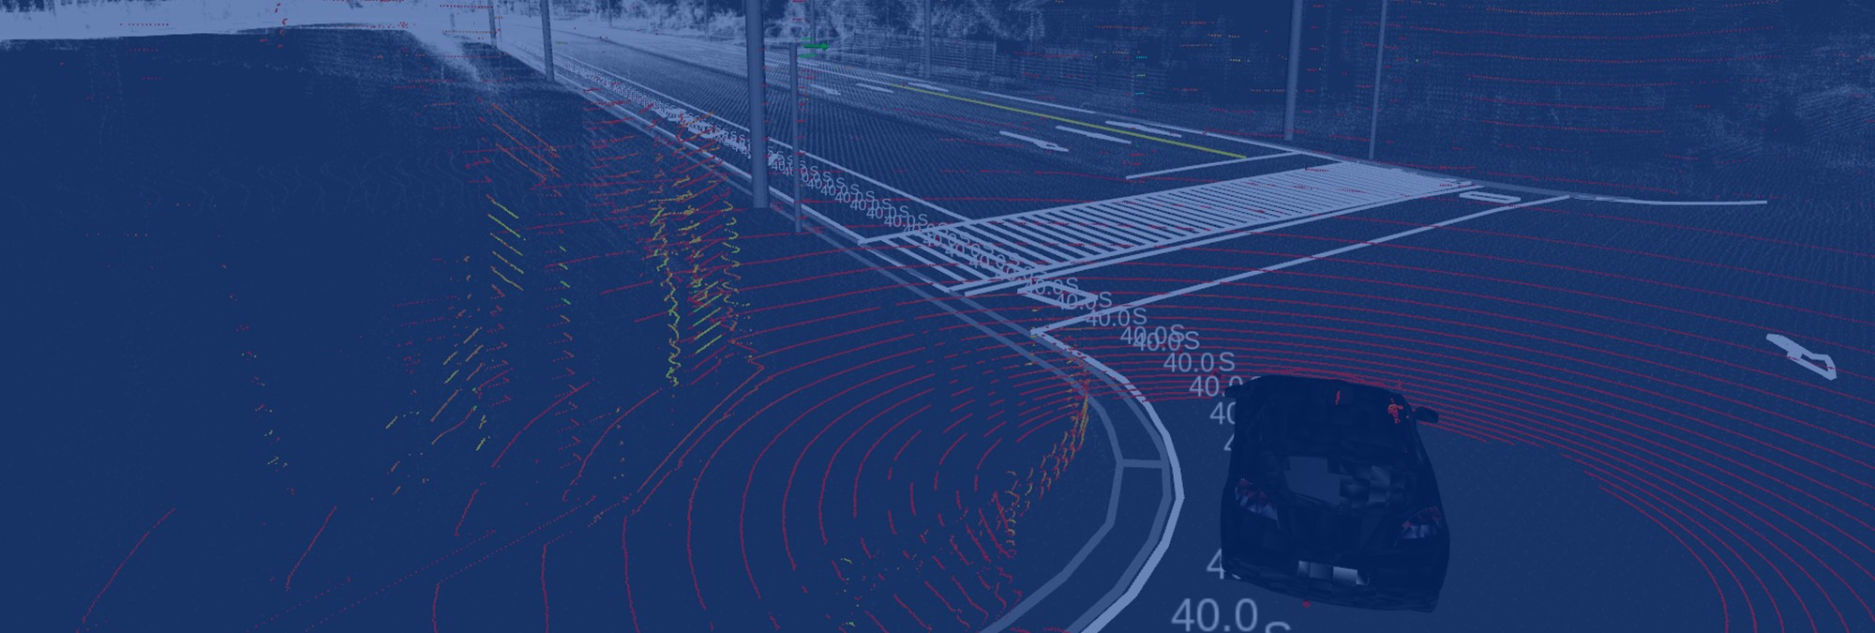
\includegraphics[scale=0.512]{\beamerDir/master_figure/last.pdf}\end{textblock*}\end{frame}}
\newcommand{\todo}[1]{\al{\LARGE\textbf{TODO:} #1}}
\newcommand{\headerheight}[0]{5mm}
\newcommand{\footerheight}[0]{5mm}
\newcommand{\slideheight}[0]{\textheight-\headerheight-\footerheight}
\newcommand{\tabml}[1]{\hspace{-2.1mm}\begin{tabular}{l} #1 \end{tabular}}
\newcommand{\al}[1]{\alert{#1}}
\newcommand{\argempty}[0]{}
\newcommand{\onlyslide}[1]{
    \vspace{\headerheight}
    \begin{minipage}[c][\slideheight][c]{\textwidth}
        #1
    \end{minipage}
}
\newcommand{\onlyimage}[1]{
    \onlyslide{
        \centering
        \begin{columns}
            \begin{column}{\textwidth}
                \centering
                \adjustbox{max width=\textwidth, max height=\slideheight}{
                    \includegraphics{#1}
                }
            \end{column}
        \end{columns}
    }
}
% fit image
\newlength\fitimageht
\newlength\fitotherht
\newsavebox\fitimagebox
\newcommand{\fitimage}[2]{%
    \sbox\fitimagebox{%
        \parbox{\textwidth}{%
            #1\par
        }%
    }%
    \settototalheight{\fitotherht}{%
        \usebox\fitimagebox
    }%
    \setlength\fitimageht{\textheight}%
    \addtolength\fitimageht{-\fitotherht-\headerheight-\footerheight-1\baselineskip}%
    \vspace{\headerheight}
    #1\par
    \centering
    \includegraphics[width=\textwidth,height=\fitimageht,keepaspectratio]{#2}
}
% Simplification
\newcommand{\assume}[1]{
    \begin{exampleblock}{Simplification }
        #1
    \end{exampleblock}
}
% Re-post
\setbeamercolor{RepostBox}{fg=black!50, bg=coolblack!10}
\newcommand{\repost}[1]{
    \vspace{2mm}
    \centering
    \begin{columns}
        \begin{column}{0.86\textwidth}
            \begin{beamercolorbox}[wd=\textwidth, sep=2pt, rounded=true, shadow=true]{RepostBox}
                \begin{tabular}{|p{0.95\textwidth}}
                    {\fontsize{10pt}{10pt}#1}
                \end{tabular}
            \end{beamercolorbox}
        \end{column}
    \end{columns}
}

% equation ballon
\tcbset{
    framebox/.style={
            enhanced,
            boxsep=0pt,       % 箱の上下左右の余白を指定
            colback=white,
            boxrule=1pt,
            colframe=#1
        },
    framebox/.default=red
}
\newcommand{\upbln}[3]{
    \tcboxmath[
        framebox=#2,
        top=0.5ex,bottom=0.5ex,    % 箱の上下の余白を指定
        left=0.5ex,right=0.5ex,    % 箱の左右の余白を指定
        overlay={
                \node[
                    above,
                    rectangle callout,                         % nodeを吹き出しの形に
                    callout absolute pointer={(frame.north)},  % 吹き出しの先端を絶対的に指定
                    fill=#2!20
                ] at ([yshift=2ex]frame.north) {\footnotesize#3};
            }
    ]{#1}
}
\newcommand{\lwbln}[3]{
    \tcboxmath[
        framebox=#2,
        top=0.5ex,bottom=0.5ex,    % 箱の上下の余白を指定
        left=0.5ex,right=0.5ex,    % 箱の左右の余白を指定
        overlay={
                \node[
                    below,
                    rectangle callout,                         % nodeを吹き出しの形に
                    callout absolute pointer={(frame.south)},  % 吹き出しの先端を絶対的に指定
                    fill=#2!20
                ] at ([yshift=-2ex]frame.south) {\footnotesize#3};
            }
    ]{#1}
}
\tcbuselibrary{theorems,skins}



%%%%% Mode %%%%%
% \newcommand{\forme}[1]{#1}
\newcommand{\forme}[1]{}


%%%%% Front Cover %%%%%
\title{Response-Time Analysis of ROS 2 Processing Chains Under Reservation-Based Scheduling}
\subtitle{Euromicro Conference on Real-Time System (ECRTS), 2019}
\author{矢野 篤志}
\date{\today}
\institute[EMBIV]{EMBIV}
\logo{\begin{textblock*}{0.1\linewidth}(2pt, 237pt)
\includegraphics[scale=0.4]{\beamerDir/master_figure/Emb_logo.pdf}\end{textblock*}}


%%%%% Document Start %%%%%
\begin{document}

\maketitle

% \summary{1}{0}
% % !TeX root = main.tex


\begin{frame}{提案の概要}
    \begin{itemize}
        \item 優先度駆動型スケジューリングによってROSのリアルタイム性能と予測可能性を大幅に改善できることを主張する
        \item 主張を裏付けるために, 優先度駆動型チェーン考慮スケジューリングに関する我々の研究をレビューし, Apex.AI が開発したオープンソースリファレンスシステムを用いた評価を行う
        \item ROS 2のリアルタイム性能を向上させるために不可欠な以下2つの課題を説明する
        \begin{itemize}
            \item マルチスレッドエグゼキュータ設計
            \item アクセラレータサポート
        \end{itemize}
    \end{itemize}
\end{frame}


\begin{frame}{Outline}
    \setbeamertemplate{section in toc}[sections numbered]
    \footnotesize\tableofcontents[hideallsubsections]
\end{frame}

% !TeX root = main.tex

\section{INTRODUCTION}
\label{sec: introduction}

\begin{frame}{}
    \begin{itemize}
        \item ロボット工学のような, 様々な分野の深い専門知識を必要とする学際的で複雑なアプリケーション領域では, 通常, 全ての, あるいはほとんどのソフトウェアをゼロから書くという選択肢はあり得ない
        \item その代わりに, ロボット工学者は, ROSのような一般的なロボット工学フレームワークで容易に利用できる, 標準機能を提供する既存のサードパーティコンポーネントの統合を採用するのが一般的である
        \item その利点は数多く, 簡単に理解できる
        \item 例えば, 複数の最新パス計画アルゴリズムと3D可視化サポートを備えた完全なナビゲーションスタックがたった1回のダウンロードで手に入るなら, なぜ新しいナビゲーションサブシステムを苦労して開発する必要があるか?
    \end{itemize}
\end{frame}

\begin{frame}{}
    \begin{itemize}
        \item 完全なロボットシステムを構築するためには, 多くの相互作用するコンポーネントを統合する必要がある
        \item ROS開発プロセスの分散型オープンソースの性質により, これらのコンポーネントは通常, 必ずしもお互いを知らない複数の独立したコンポーネント開発者によって分離して開発される
        \item 同様に, システムインテグレータは, アプリケーションおよびミッション固有のロジックと「グルーコード」で展開プラットフォーム上で選択したコンポーネントを構成するが, 通常, それぞれのコンポーネント開発者と密接に連携することはない
    \end{itemize}
\end{frame}

\begin{frame}{}
    \begin{itemize}
        \item コンポーネントの統合を可能な限りシンプルに保つために, ROSはコンポーネントの疎結合を可能にする古典的なトピックベースのpublish/subscribeパラダイムを採用している
        \item 概念的には, 各コンポーネントは, 特定のトピックをsubscribeする多数のコールバックを含む「ブラックボックス」として理解できる
        \item 与えられたトピックに関連するメッセージがpublishされるたびに, 全てのsubscribeコールバックが呼び出され, 何らかの計算を実行し, 次に他のトピックに後続のメッセージをpublishすることができ, これがさらにコールバックをトリガするというように, 繰り返す
    \end{itemize}
\end{frame}

\begin{frame}{}
    \begin{itemize}
        \item インテグレータは, あるコンポーネントの「入力コールバック」を別のコンポーネントの「出力トピック」に接続することによってコンポーネントを構成する
        \item ROSシステムは, このように相互接続されたトピックとコールバックの複雑なネットワークを形成し, データ (環境刺激など) は, イベント駆動型の方法でネットワークを通じてcause-effectチェーンに沿って伝播し, インテグレータが望むように透過的にコンポーネント境界を交差させることができる
    \end{itemize}
\end{frame}

\begin{frame}{}
    \begin{itemize}
        \item このようなcause-effectチェーンの典型的な例として, 進路上の障害物を検知して反応する必要のある移動ロボットのセンシング-計算-行動パイプラインが挙げられる
        \item 例えば, ハードウェアドライバコンポーネントがレーザースキャナから新しいサンプルを取得し (cause) , それが複数のマッピング, 座標変換, パス計画, 車輪制御コンポーネントを経て, 最終的に車輪速度の変化 (effect) をもたらす可能性がある
        \item このようなデータ処理のチェーンにおいて, causeからeffectまでの最大レイテンシ時間は, ロボットが正しく機能するために重要な役割を果たすことは明らかであり, また, 安全性を考慮する上でも重要であることが多い
    \end{itemize}
\end{frame}

\begin{frame}{}
    \begin{itemize}
        \item 重要なのは, システムインテグレータにできるだけ多くの展開の選択肢を残し, コンポーネントの再利用の機会を最大化するために, ROSの実行管理層と基礎となるオペレーティングシステムは, 意図的にコンポーネント開発者に公開されないことである
        \item むしろ, ROSの中心的なコールバック抽象化は, コールバック手続きがいつどのようにスケジュールされるか, コールバックの実行がスレッドまたはプロセスにわたってどのように組織されるか, またはネットワーキング層がメッセージの送受信をどのように処理するかを全く意識せずに, 実行から完了までセマンティクスを持つ単なる手続きである
    \end{itemize}
\end{frame}

\begin{frame}{}
    \begin{itemize}
        \item ROSはオープンソースソフトウェアであるため, 原理的にはシステムの実行と通信の挙動を完全に理解し制御することが可能である
        \item このため, リアルタイムシステムの専門家から見れば, ROSにリアルタイムシステム研究でよく知られた技術を導入することは論理的なステップであるように思える可能性がある
        \item しかし, 一見したところ, これを難しくしているハードルがいくつかある
    \end{itemize}
\end{frame}

\begin{frame}{}
    \begin{itemize}
        \item まず第一に, インテグレータに必要な情報が不足している
        \item ほとんどのリアルタイム分析では, 同時実行タスクの数, それらの起動セマンティクスや機能的相互作用, メッセージの到着パターン, 最悪実行時間など, 多くの低レベルシステムの詳細に関する深い知識が前提となっている
        \item ROSコンポーネントは, この種の情報を提供するマニフェストと一緒に来ることはない
        \item さらに悪いことに, リアルタイム分析は, 欠陥のある情報や不完全な情報にうまく対処できない
        \item モデリング目的でサードパーティコンポーネントを手作業でリバースエンジニアリングしているときに, たった一つのミスや見落としがあれば, その取り組み全体を無条件に無効にしてしまうことになりかねない
    \end{itemize}
\end{frame}

\begin{frame}{}
    \begin{itemize}
        \item 第二に, 必要なシステムの詳細をコンポーネントレベルで静的に決定し, 記述することができない
        \item その理由のひとつは, 多くのロボット工学アルゴリズムが, ユースケースやプラットフォーム固有の側面に依存し, 実行時間や起動パターンが大きく変化するためである
        \item 例えば, ビデオストリーム中の物体を識別し, その軌跡を推測する一般的な物体追跡コンポーネントを考えてみよう (例えば, 隣の車線の車など)
        \item この機能の実行時間は, ビデオストリームのフレームレート, 解像度, コーデック, および特定のトラッキングアルゴリズムに関連する他の様々なパラメータを含む, 様々なパラメータに依存する
        \item これらのパラメータは, 一般的なオブジェクトトラッキングコンポーネントの開発者が前もって知っていたり, 固定されていたりするものではない
    \end{itemize}
\end{frame}

\begin{frame}{}
    \begin{itemize}
        \item このようなユースケース特有の情報は, 特定のロボットを構築するインテグレーターにしか分からない
        \item インテグレーターは, 必ずしもオブジェクトトラッキングやリアルタイムシステムの専門家ではないため, 特定の構成を選択した場合の影響を常に予測できるわけではない
        \item したがって, コンポーネントのリソース要求とリアルタイム動作は, 常に特定の展開で使用するという文脈で評価されなければならない
        \item これは, ROSフレームワークの人気の根底にある「ブラックボックス」コンポーネントのモジュール式再利用と相容れるものではない
    \end{itemize}
\end{frame}

\begin{frame}{}
    \begin{itemize}
        \item 最後に, 仮にインテグレータが各コンポーネントについてそれぞれの専門家と議論し, タイミング分析に必要な全ての詳細を入手できたとしても, 第三の根本的な問題が残る
        \item 多くのコンポーネントのリソース要件と性能特性は, 本質的にロボットの動的環境に依存し, したがって時間とともに変化するため, 静的 (最悪のケース) リソース配置は実行不可能なのである
    \end{itemize}
\end{frame}

\begin{frame}{}
    \begin{itemize}
        \item 例えば, 前述の物体追跡コンポーネントと, ランドマークベースの自己位置特定コンポーネントに依存するロボットを再度考えてみよう
        \item 一方, 人口が少ない田舎町よりも, にぎやかな街中を移動する方が, 物体追跡装置の処理時間はずっと長くなる
        \item 一方, 認識可能なランドマークが多い都市部では, ほぼ一様な風景よりも自己位置推定がはるかに容易である可能性が高い
        \item どちらの状況でも十分なリソースを確保するためには, システムインテグレーターは, 不毛の土地からなる賑やかな都市を想定したシステムを用意しなければならない
    \end{itemize}
\end{frame}

\begin{frame}{}
    \begin{itemize}
        \item ロボット工学では, このような悲観的なシステム設計を行うと, すぐに現実的な限界に直面することになる
        \item その代わりに, 実用的で費用対効果の高いシステムを維持するためには, 各コンポーネントのピーク需要の合計ではなく, 予想されるジョイントリソースのピーク需要に対してプロビジョニングを行う必要がある
    \end{itemize}
\end{frame}

\begin{frame}{貢献する}
    \begin{itemize}
        \item これらの課題を克服するために, 我々は, 実行時に動的にタイミングを考慮した方法でROSシステムをプロビジョニングするための自動レイテンシマネージャを使用することを提案する
        \item 具体的には, ROS Live latency manager (ROSLlama) を紹介する
        \item これは, 重要なcause-effectチェーンに沿ったレイテンシを, 非リアルタイム専門家が使いやすく, かつ設定にあまり手間をかけない方法で, 既存のリアルタイム機構を使用して制御することを可能にする
    \end{itemize}
\end{frame}

\begin{frame}{貢献する}
    \begin{itemize}
        \item ROS-Llamaは, 複雑なシステムパラメータをユーザに要求するのではなく, 実行時に必要なパラメータを自動的に推定し, 状況の変化に応じてスケジューリングパラメータを動的に調整することが可能である
        \item もし, 指定されたレイテンシの目標が全て同時に達成できない場合 (例えば, 不利な環境条件による一時的な過負荷が原因) , ROS-Llamaは制御された緩やかなデグレードプロセスを開始し, システムインテグレーターが純粋に宣言的な方法で (すなわち, cause-effectチェーンがどの部品を通過しているかを理解しなくても) cause-effectチェーンの重要性を特定できるようにする
    \end{itemize}
\end{frame}

\begin{frame}{本論文の貢献}
    \begin{itemize}
        \item  ロボティクス領域における動的レイテンシ管理問題を探求し, 実用的なソリューションが満たさなければならない制約と要件を文書化する (第III章)

        \item  ROSのための最初の自動レイテンシマネージャであるROS-Llamaの設計と実装を紹介する (セクションIV)

        \item 標準的な Linux システム上の ROS コンポーネントを用いて, ROS-Llama が移動ロボットのcause-effectチェーンのレイテンシをうまく制御できることを示す評価について報告する (セクションVI)

    \end{itemize}
\end{frame}

\begin{frame}{}
    \begin{itemize}
        \item ROS-Llamaは, 数年にわたる研究とエンジニアリングの努力の結果であり, その間, 我々は多くの課題や技術的な限界に遭遇した
        \item セクションVIIでは, 以下の点を強調する
              \begin{itemize}
                  \item  ROS-Llamaをより効果的かつ正確にするための分析改善の機会
                  \item  ROSとLinuxのプラットフォームには, システムのさらなる改良の妨げとなる大きな限界がある
              \end{itemize}
    \end{itemize}
\end{frame}
 % wait kobayu
% !TeX root = main.tex


\section{BACKGROUND}
\label{sec: background}


\subsection{ROS2}
\label{ssec: ros2}

\begin{frame}{ROS 2}
    \fitimage{
        \al{ROS 2} は OS 上の複数の抽象化レイヤの統合実装
    }{figure/ros2_system.png}
\end{frame}

\begin{frame}{Publish/Subscribeパラダイム}
    ROS 2 アプリケーションは, \al{publish/subscribeパラダイム}を使用して相互に通信する複数のノードで構成される

    \begin{block}{Publish/Subscribeパラダイム}
        \setlength{\linewidth}{0.98\columnwidth}
        \begin{itemize}
            \item ノードはトピックにメッセージをpublishし, そのトピックをsubscribeしているノードにメッセージをブロードキャストする
            \item ノードはコールバックをアクティブにして各メッセージを処理することにより, publish メッセージに反応する
            \item コールバックはメッセージ自体をpublishすることも可能で, 複雑な動作をトピックとコールバックのネットワークとして実装できる
        \end{itemize}
    \end{block}
\end{frame}

\begin{frame}{エグゼキュータ}
    \begin{itemize}
        \item ROS 2 アプリケーションがプラットフォームに展開される際には, 個々のノードが OS のプロセスにマップされる
        \item ROS 2 クライアントライブラリの\al{エグゼキュータ}は, OS プロセス内のノードのコールバックの実行を調整する
    \end{itemize}
\end{frame}

\begin{frame}{シングル/マルチスレッドエグゼキュータ}
    \begin{itemize}
        \item ROS 2 には以下 \tu{2 つの組み込みエグゼキュータがある}
              \begin{block}{シングルスレッドエグゼキュータ}
                  1 つのスレッドでコールバックを実行するエグゼキュータ
              \end{block}
              \begin{block}{マルチスレッドエグゼキュータ}
                  コールバックの処理を複数のスレッドに分散するエグゼキュータ
              \end{block}
              \vspace{5mm}

        \item \textbf{\underline{本論文ではマルチスレッドエグゼキュータに焦点を当てる}}
    \end{itemize}
\end{frame}

\begin{frame}{DDS (Data Distribution Service)}
    ノードのpublisherとsubscriberの間のメッセージ交換は, 抽象\al{DDS} (Data Distribution Service) 層によって実現される

    \begin{block}{抽象DDS}
        DDS とクライアントライブラリ間の通信インタフェース
    \end{block}
    \begin{block}{DDS}
        publisherとsubscriber間でメッセージを交換するための業界標準の分散通信システム
    \end{block}
\end{frame}

\begin{frame}{処理チェーン}
    \fitimage{
        \begin{itemize}
            \item \al{処理チェーン}は特定のイベントによってトリガされ, 複数のエグゼキュータにまたがる
            \item チェーンの各頂点はコールバックを表す
        \end{itemize}
    }{figure/multi_threaded_executor.png}
\end{frame}

\begin{frame}{本論文の分析の焦点}
    \fitimage{
        \tu{本論文では単一のエグゼキュータにおけるチェーンの応答時間に焦点を当てる}
        \notes{CPAアプローチ*によってチェーンが複数のエグゼキュータにまたがる場合に拡張できる}
    }{figure/multi_threaded_executor.png}

    \source{*D.Casini et al., “Response time analysis of ROS 2 processing chains under reservation-based scheduling,” in ECRTS, 2019.}
\end{frame}

\begin{frame}{コールバックグループ}
    \fitimage{
        \begin{itemize}
            \item コールバックは必ず1つの\al{コールバックグループ}に属す
            \item エグゼキュータ内のコールバックは, 異なるコールバックグループに属す可能性がある
        \end{itemize}
    }{figure/multi_threaded_executor.png}

\end{frame}

\begin{frame}{ノード}
    \begin{itemize}
        \item コールバックは異なる\al{ノード}に属す場合もある
        \item ROS 2 では, 同じノード内のコールバックはデフォルトで同じコールバックグループとなる
        \item これを除いて, ノードの概念は本論文とは無関係
    \end{itemize}

    \assume{簡単にするために, モデルにノードレベルの情報を含めない}
\end{frame}


\subsection{Scheduling of multi-threaded executor}
\label{ssec: scheduling_of_multi_threaded_executor}

\begin{frame}{}
    \begin{itemize}
        \item ROS 2 マルチスレッドエグゼキュータのスケジューリング動作を紹介する
        \item \tu{本論文の内容は ROS 2 Foxy Fitzroy に基づいている}
    \end{itemize}

\end{frame}

\begin{frame}{コールバック}
    \begin{itemize}
        \item \al{コールバック}は ROS 2 の最小のスケジューリングエンティティ
        \item マルチスレッドエグゼキュータでは, スレッドは抽象 DDS レイヤからメッセージを受け取り, 対応するコールバックを実行する
    \end{itemize}
\end{frame}

\begin{frame}{コールバックの優先順位決定方法}
    ROS 2 では, \tu{コールバックの優先度は 2 つのレベルで決定される}

    \begin{block}{コールバックタイプ}
        \setlength{\linewidth}{0.98\columnwidth}
        \begin{itemize}
            \item コールバックはタイマ・サブスクライバ・サービス・クライアントの 4 つのタイプに分類される
            \item 優先順位は, タイマ $\succ$ サブスクライバ $\succ$ サービス $\succ$ クライアント \notes{$\succ$: より高い優先度を持つ}
        \end{itemize}
    \end{block}

    \begin{block}{登録順}
        先に登録されたコールバックが優先される
    \end{block}
\end{frame}

\begin{frame}{コールバックタイプに関する簡単化}
    \full{
        \assume{本論文ではコールバックタイプに関する情報は含めない}
    }
\end{frame}

\begin{frame}{yield\_before\_execute}
    \begin{itemize}
        \item \al{yield\_before\_execute} が false に設定されている場合, スレッドは選択されたコールバックの実行をすぐに開始する
        \item yield\_before\_execute が true に設定されている場合, スレッドは再度スケジュールされるまでプロセッサを OS に譲る
        \item \tu{本論文ではデフォルトの設定である yield\_before\_execute $=$ false とする}
    \end{itemize}
\end{frame}

\begin{frame}{メッセージキュー}
    ROS 2 では, 各コールバックに到着したメッセージをバッファリングするためのキューがあり, その深さはユーザによって指定される
    \assume{
        \setlength{\linewidth}{0.98\columnwidth}
        \begin{itemize}
            \item キューが十分に大きく, メッセージが上書きされない
            \item コールバックは最も早く到着したメッセージでノンプリエンプティブに実行される
        \end{itemize}
    }
\end{frame}

\begin{frame}{wait\_set}
    エグゼキュータ内のスレッドは共通のセット \al{wait\_set} によって, 利用可能なメッセージを持つコールバックを保持する
\end{frame}

\begin{frame}{reentrant/mutually exclusiveコールバックグループ}
    \tu{コールバックグループには以下2つの種類がある}
    \begin{block}{Reentrantコールバックグループ}
        wait\_set内のコールバックはいつでも選択できる
    \end{block}
    \begin{block}{Mutually exclusiveコールバックグループ}
        \setlength{\linewidth}{0.98\columnwidth}
        \begin{itemize}
            \item 各グループに排他制御フラグ \al{can\_be\_taken\_from} がある
            \item グループのコールバックが選択されるとフラグは false に設定され, コールバックの終了後に true に設定される
            \item mutually exclusive コールバックグループに属すコールバックは,  can\_be\_taken\_from が true の場合にのみ選択できる
        \end{itemize}
    \end{block}
\end{frame}

\begin{frame}{スレッドのワークフロー全体像}
    \fullimage{figure/thread_workflow.png}
\end{frame}

\begin{frame}{[ワークフロー] low\_priority\_wait\_mutex}
    \fitimage{
        \begin{itemize}
            \item スレッドは wait\_set にアクセスする前に, 排他制御ロック \al{low\_priority\_wait\_mutex} を獲得する必要がある
            \item すなわち wait\_set を変更できるのは一度に 1 つのスレッドのみ
            \item それ以外の場合, スレッドはブロックされる
        \end{itemize}
    }{figure/workflow1.jpg}
\end{frame}

\begin{frame}{[ワークフロー] mutually exclusiveコールバックグループの挙動1}
    \fullimage{figure/workflow2.jpg}
\end{frame}

\begin{frame}{[ワークフロー] コールバック選択後}
    \fitimage{
        コールバックが選択されると, スレッドは wait\_set からコールバックを削除し, low\_priority\_wait\_mutex をリリースする
    }{figure/workflow4.jpg}
\end{frame}

\begin{frame}{[ワークフロー] mutually exclusiveコールバックグループの挙動2}
    \fullimage{figure/workflow3.jpg}
\end{frame}


\begin{frame}{[ワークフロー] コールバックが選択できない場合}
    \fitimage{
        \begin{itemize}
            \item 全てのコールバックがチェックされ, 実行するコールバックを選択できない場合, スレッドは wait\_set をリセットし, wait\_set を更新する
            \item mutually exclusive コールバックグループのコールバックは, can\_be\_taken\_from が true の場合にのみ wait\_set に追加できる
        \end{itemize}
    }{figure/workflow5.jpg}
\end{frame}

\begin{frame}{[ワークフロー] コールバックを wait\_set に追加できない場合}
    \begin{columns}
        \begin{column}{0.4\textwidth}
            コールバックを wait\_set に追加できない場合, スレッドは low\_priority\_wait\_mutex をリリースしてアイドル状態になる
        \end{column}
        \begin{column}{0.6\textwidth}
            \fullimage{figure/workflow6.jpg}
        \end{column}
    \end{columns}
\end{frame}

% !TeX root = main.tex

\section{ROS Scheduling}
\label{sec: ros scheduling}


\begin{frame}{セクションサマリ}
    \begin{itembox}[l]{\textbf{目的}}
        ROS のスケジューリング動作を包括的に説明する
    \end{itembox}
\end{frame}

\begin{frame}{}
    \begin{itemize}
        \item エグゼキューターは, コールバックの 4 つのカテゴリを区別する.システムレベルのタイマーによってトリガされるタイマー, サブスクライブされたトピックの新しいメッセージによってトリガされるサブスクライバー, サービス要求によってトリガされるサービス, および応答によってトリガされるクライアントである.サービスリクエスト.エグゼキューターは, ($r c l$ レイヤーと対話することによって) DDS レイヤーの入力キューからメッセージを取得し, 対応するコールバックを実行する責任がある.完了までコールバックを実行するため, 非プリエンプティブ スケジューラである.
    \end{itemize}
\end{frame}

\begin{frame}{}
    \begin{itemize}
        \item ただし, 最も一般的に研究されているスケジューラとは異なり, 実行可能なすべてのタスクを常に考慮しているわけではない.代わりに, readySet に基づいて決定する.これは, 実行に依存する不規則な間隔で更新される, 準備完了の非タイマー コールバックのセットのキャッシュされたコピーである.
    \end{itemize}
\end{frame}

\begin{frame}{アルゴリズム2}
    \fullimage{thread_flow}
\end{frame}

\begin{frame}{}
    \begin{itemize}
        \item エグゼキュータがアイドル状態の場合, readySet を更新する.これは, エグゼキュータが基礎となる通信層 (つまり,  $r c l$ を介した rmw) と対話する唯一のステップである.次に, 4 つのコールバック カテゴリを検索して, 実行するコールバックを探する (効率のために, 何もすることがない場合, エグゼキュータはブロックする.この最適化は, わかりやすくするために省略されている).最初に, タイマーがデッドライン切れになっているかどうかを確認する.これらは DDS レイヤーによって管理されないため, このチェックは現在のタイマーの状態に基づいており, readySet には依存しない.
    \end{itemize}
\end{frame}

\begin{frame}{}
    \begin{itemize}
        \item 次に, readySet でサブスクリプション, サービス, クライアントを (この順序で) 検索する.固定された順序でキューを評価すると, 各キューに異なる優先度が割り当てられるという本質的な効果がある (つまり, タイマー キューが最初に検査されるため, 優先度が最も高くなり, クライアント キューが最後に検査され, 優先度が最も低くなる).キューが考慮される場合, コールバック インスタンスは, コールバックの登録順, つまり, コールバックがエグゼキュータに登録された順序で検査される.したがって, 登録順序は, 第 2 レベルの優先度を表す.全体として, ペア (コールバック タイプ, 登録時間) は, 各コールバックの固有の優先順位である.
    \end{itemize}
\end{frame}

\begin{frame}{}
    \begin{itemize}
        \item カテゴリに少なくとも 1 つの準備完了コールバックがある場合は常に, 最も優先度の高いコールバックが選択され, 実行されてから, readySet から削除される.最後に, readySet が空で, デッドライン切れのタイマーが残っていない場合, executor はアイドル状態に戻り, 通信レイヤーの現在のスナップショットに基づいて readySet を更新する. readySet の更新をポーリング ポイントと呼び, 2 つのポーリング ポイント間の間隔を処理ウィンドウと呼びます.
    \end{itemize}
\end{frame}

\begin{frame}{}
    \begin{itemize}
        \item 通常の固定優先度スケジューリングと比較すると, このアルゴリズムにはいくつかの変わった特性がある.まず, 処理ウィンドウ中に到着したメッセージは, 残りのすべてのコールバックに依存する次のポーリング ポイントまで考慮されない.これは, 優先度の低いコールバックが現在の処理ウィンドウを引き延ばすことによって, 優先度の高いコールバックを暗黙的にブロックする可能性があるため, 優先度の逆転につながります.
    \end{itemize}
\end{frame}

\begin{frame}{}
    \begin{itemize}
        \item 第 2 に, より一般的なレディ リストではなく, レディ セットに依存する.これは, タイマー以外のコールバックのインスタンスがいくつ用意されているかをアルゴリズムが認識できないことを意味する.したがって, 処理ウィンドウごとに任意のコールバックのインスタンスを最大 1 つ処理する.これにより, 上記の優先度の逆転が悪化する.バックログされたコールバックは, スケジューリングが考慮されるまで複数の処理ウィンドウを待機する必要がある場合があるためである.事実上, これは非タイマー コールバック インスタンスが同じ優先度の低いコールバックの複数のインスタンスによってブロックされる可能性があることを意味する.
    \end{itemize}
\end{frame}

\begin{frame}{}
    \begin{itemize}
        \item ROS スケジューラの説明は, 手動のコード検査に基づいている.ただし, ROS のような複雑なシステムでは, これは潜在的にエラーが発生しやすくなる.これは, 簡単に見落とされがちな微妙な相互作用があり, 動作を大幅に変更する可能性があるためである.したがって, モデルを検証するために, 結果のトレースから ROS スケジューラの動作を推測できるように, 任意の長さのコールバックを実行する特別な目的の ROS ノードを実装した.具体的には, ノードは 3 つのトピック $(H, M$ および $L)$, 3 つのサービス $(S H, S M$ および $S L$ ), およびタイマーを作成するための専用のトピックを使用して制御される.選択された名前は, トピックとサービスが登録順に優先されることを想定していることに注意.トピック $H$ が実際に最高の優先度を持っていることを確認することは, モデル検証の一部である.
    \end{itemize}
\end{frame}

\begin{frame}{}
    \begin{itemize}
        \item 以下の説明では, タイム ゼロは, 検証コールバックの最初のバッチがノードに到着した時点を指す. $i$ 番目のタイマーは $t_{i}$ として示される.視覚化を容易にするために, すべてのコールバックは $500 \mathrm{~ms}$ に対して実行される.
    \end{itemize}
\end{frame}

\begin{frame}{}
    \begin{itemize}
        \item このテストでは, 最初に $200 \mathrm{~ms}\left(T_{0}\right)$ で 2 つのタイマーをセットアップし, $2300 \mathrm{~ms}\left(T_{3}\right)$ で 2 つのタイマーをセットアップする.次に, メッセージ シーケンス $<L M H S H S L L M H S H S L>$ を送信し, $1.5$ 秒間 $\left(T_{2}\right)$ 待機してから, $\angle S M S M H\rangle$ を送信する.結果を図 3 に示す.ポーリング ポイントはテストによって決定されないことに注意.むしろ, 結果のタイミング動作から推測される.
    \end{itemize}
\end{frame}

\begin{frame}{}
    \begin{itemize}
        \item 複数のメッセージがキューに入れられていても, スケジューラーが準備完了イベントごとに 1 つのコールバックのみを実行していることを明確に確認できる.これは, 2 番目のポーリング ポイントの後で特に顕著である.さらに, SM は $T_{2}$ に早く到着したとしても (つまり,  $t_{1}$ の実行中に), 時間 4 で明らかにスキップされる.これにより, ポーリング ポイントの存在が証明される.ただし, $t_{2}$ と $t_{3}$ は $S M$ より遅れて到着するが, 最初の処理ウィンドウ中に実行されるため, タイマーは明らかにこれらのポーリング ポイントの影響を受けません.
    \end{itemize}
\end{frame}
 % wait kobayu
% % !TeX root = main.tex

\section{PRIOR KNOWLEDGE}
\label{sec: prior knowledge}

\begin{frame}{前提知識}
    \begin{itemize}
        \item \ourl{ROS}{https://tier4.atlassian.net/wiki/spaces/EMBIV/pages/2683603071/ROS+Robot+Operating+System}
        \item \ourl{publish/subscribeモデル}{https://tier4.atlassian.net/wiki/spaces/EMBIV/pages/2675048610/Publish+Subscribe}
        \item \ourl{SCHED\_DEADLINE}{https://tier4.atlassian.net/wiki/spaces/EMBIV/pages/2692645566/SCHED+DEADLINE}
        \item \ourl{最大イベント到着曲線}{https://drive.google.com/file/d/1n85X0vDrDm4IDANDP4aUoC0SNnZLAiRN/view?usp=share_link}
        \item \ourl{Casiniらによる先行研究}{https://drive.google.com/file/d/1sHujFqbmgCoJbC6g6KdC7ihua4Jqddju/view?usp=share_link}
    \end{itemize}
\end{frame}

% % !TeX root = main.tex

\section{SYSTEM MODEL}
\label{sec: system_model}


\begin{frame}{}
    以下では, 上記の説明から抽出したマルチスレッドエグゼキュータのリアルタイム関連の動作をカバーするスケジューリングモデルを紹介する
\end{frame}

\begin{frame}{}
    \assume{簡単にするために, wait\_set にアクセスまたは更新するスレッドによって発生するオーバヘッドはゼロであると仮定する}
\end{frame}

\begin{frame}{Notations1}
    \begin{table}[tb]
        \adjustbox{max width=\textwidth, max height=\slideheight}{
            \centering\begin{tabular}{|c|l|} \hline
                \textbf{Notations}      & \textbf{Descriptions}                                                                       \\\hline
                $C_i$                   & チェイン                                                                                    \\\hline
                $m$                     & スレッド数                                                                                  \\\hline
                $\Gamma $               & チェインのセット                                                                            \\\hline
                $c_{i,j}$               & $C_i$の$j$番目のコールバック                                                                \\\hline
                $e_{i,j}$               & $c_{i,j}$のWCET                                                                             \\\hline
                $E_i$                   & $C_i$内のコールバックのWCETの合計                                                           \\\hline
                $D_i$                   & $C_i$のデッドライン                                                                         \\\hline
                $T_i$                   & $C_i$の周期                                                                                 \\\hline
                % $U_i$                   & $C_i$の利用率                                                                               \\\hline
                % $\mathcal{G}(c_{i,j}) $ & $c_{i,j}$が属すmutually exclusiveコールバックグループのインデックス                         \\\hline
                $\theta_i$              & \tabml{$\mathcal{C}_{i}$ の各コールバックが属すmutually exclusiveコールバックグループの集合 \\ $\theta_{i}=\cup_{\forall c_{i, j} \in \mathcal{C}_{i}}\left\{\mathcal{G}\left(c_{i, j}\right)\right\}$} \\\hline
            \end{tabular}
        }
    \end{table}
\end{frame}

\begin{frame}{Notation2}
    \begin{table}[tb]
        \adjustbox{max width=\textwidth}{
            \centering\begin{tabular}{|c|l|} \hline
                \textbf{Notations} & \textbf{Descriptions}                                       \\\hline
                $J_{i}^{k}$        & $\mathcal{C}_{i}$ の $k$番目のインスタンス                  \\\hline
                $c_{i, j}^{k}$     & $J_{i}^{k}$ に含まれる$c_{i, j}$ のコールバックインスタンス \\\hline
            \end{tabular}
        }
    \end{table}
\end{frame}

\subsection{Workload Model}
\label{ssec: workload_model}

\begin{frame}{チェーンの定義}

    \begin{itemize}
        \item $m$ スレッド上のマルチスレッドエグゼキュータによってスケジュールされた一連の独立した処理チェーン (略してチェーンと呼ぶ) $\Gamma=\left\{\mathcal{C}_{1}, \mathcal{C}_{2}, \cdots, \mathcal{C}_{|\Gamma|}\right\}$ を検討する

              \assume{各スレッドは専用プロセッサに静的に展開されており,スレッドはいつでもプロセッサを使用できる}

        \item 各チェーン $\mathcal{C}_{i} \in \Gamma$ は, コールバック $\mathcal{C}_{i}=\left\{c_{i, 1}, c_{i, 2}, \cdots, c_{i,\left|\mathcal{C}_{i}\right|}\right\}$ の順序付けられたシーケンスで構成される
        \item $\mathcal{C}_{i}$ の最初のコールバック $c_{i, 1}$ (それぞれ, 最後のコールバック $c_{i,\left|\mathcal{C}_{i}\right|}$ ) は, $\mathcal{C}_{i}$ のソースコールバック (それぞれ, シンクコールバック) と呼ばれる
    \end{itemize}
\end{frame}

\begin{frame}{}
    \begin{itemize}
        \item 各コールバック $c_{i, j}$ は最悪実行時間 (WCET) $e_{i, j}$ によって特徴付けられる
        \item コールバックは, 固有のmutually exclusive コールバックグループまたはreentrant コールバックグループのいずれかに属している
    \end{itemize}
\end{frame}

\begin{frame}{}
    \begin{itemize}
        \item チェーン $\mathcal{C}_{i}$ は, チェーンインスタンスの無限シーケンスをリリースする
        \item $T_{i}$ の周期は, $\mathcal{C}_{i} \cdot \mathcal{C}_{i}$ の 2 つの連続するチェーンインスタンスのリリース時刻の間の最小間隔
        \item 相対デッドライン $D_{i}$ があり, 時間 $r$ でリリースされた $\mathcal{C}_{i}$ の各チェーンインスタンスは, その絶対デッドライン $r+D_{i}$ までに終了する必要がある
        \item チェーンには制約付きデッドライン, つまり $D_{i} \leq T_{i}$ があると想定している
        \item $\mathcal{C}_{i}$ の利用率は $U_{i}=E_{i} / T_{i}$ である
    \end{itemize}
\end{frame}

\begin{frame}{}
    \begin{itemize}
        \item $J_{i}^{k}$ 内の連続する要素 $c_{i, j}^{k}$ と $c_{i, j+1}^{k}$ の各ペアについて, $c_{i, j}^{k}$ を $c_{i, j+1}^{k}$ の先行要素, $c_{i, j+1}^{k}$ を $c_{i, j}^{k}$ の後続要素と呼ぶ
        \item 非シンクコールバックインスタンス $c_{i, j}^{k}$ が実行を終了すると, 後続のインスタンスを呼び出すメッセージが生成される
    \end{itemize}
\end{frame}

\begin{frame}{応答時間の定義}
    \begin{itemize}
        \item 応答時間 $R\left(J_{i}^{k}\right)$ は,  $J_{i}^{k}$ のリリース時刻と終了時間の間の時間間隔である
        \item チェーン $\mathcal{C}_{i}$ の最悪応答時間 $\mathcal{R}_{i}^{w c}$ は, そのすべてのインスタンスの中で最大の応答時間である
        \item チェーンは, そのすべてのインスタンスがデッドラインを満たしている場合 (つまり, $\mathcal{R}_{i}^{w c} \leq D_{i}$), スケジュール可能であると言われ, $\Gamma$ は, すべてのチェーンがスケジュール可能である場合 (つまり, $\forall i: \mathcal{R}_{i}^{w c} \leq D_{i}$), スケジュール可能であると呼ぶ
    \end{itemize}
\end{frame}

\begin{frame}{本論文の目的}
    この論文の目的は, システム $\Gamma$ がマルチスレッドエグゼキュータでスケジュール可能かどうかを判断し, $\Gamma$ がスケジュール可能である場合, 各チェーン $\mathcal{C}_{i} \in \Gamma$ の $\mathcal{R}_{i}^{w c}$ の安全な上界を計算することである
\end{frame}


\subsection{Scheduling Model}
\label{ssec: scheduling_model}


\begin{frame}{}
    \begin{itemize}
        \item 実行時に, $J_{i}^{k}$ 内の最初のコールバックインスタンス $c_{i, 1}^{k}$ は, $J_{i}^{k}$ がリリースされるときにリリースされる
        \item $J_{i}^{k}$ 内の別のコールバックインスタンスは, その先行の終了時, つまり, 先行からの入力メッセージが利用可能になった時点でリリースされる
        \item 同じコールバックの複数のインスタンスがリリースされた場合、リリース時刻を基準にFIFOにエンキューされる
    \end{itemize}
\end{frame}

\begin{frame}{Pending}


    \begin{itemize}
        \item コールバックインスタンス$c_{i, j}$は、それがリリースされ、その前のインスタンスがすべて実行中か終了しているとき、\al{pending} と呼ぶ
        \item pendingコールバックインスタンス$c_{i, j}$は、\al{ready} または\al{P-blocked} のいずれかである
              \begin{itemize}
                  \item  $c_{i, j}$ がmutually exclusive コールバックグループに属している場合, $c_{i, j}$ と同じコールバックグループ内のコールバックのインスタンス ($c_{i, j}$ 自体を含む) が実行されていない場合, $c_{i, j}$ はreadyである
                  \item それ以外の場合, $c_{i, j}$ は P-blockedされる

                  \item  $c_{i, j}$ が再入可能コールバックグループに属している場合, pending $c_{i, j}$ は常に ready である
              \end{itemize}
    \end{itemize}
\end{frame}

\begin{frame}{$\Omega$}
    エグゼキュータは, 実行のために選択できるreadyコールバックインスタンスを記録するreadyセット $\Omega$ を持っている
\end{frame}

\begin{frame}{Eligible}
    \begin{itemize}
        \item $\Omega$ 内の ready のコールバックインスタンス $c_{i, j}$ が選択されるための前提条件は, \al{eligible} であることである
        \item mutually exclusive コールバックグループに属す $\Omega$ 内のコールバックインスタンス $c_{i, j}$ は, $c_{i, j}$ と同じコールバックグループ内のコールバックのインスタンスが実行されていない場合に eligible であり, それ以外の場合は \al{R-blocked} される
        \item 対照的に, reentrant コールバックグループに属すコールバックインスタンスは, $\Omega$ にある場合は常に eligible である
        \item つまり, いつでも, $\Omega$ のコールバックインスタンスは eligible であるか, R-blockedされている
        \item つまり, mutually exclusive同じコールバックグループ内のコールバックのコールバックインスタンスは, 並列に実行されることは決してない
    \end{itemize}
\end{frame}

\begin{frame}{updated, poling point}
    \begin{itemize}
        \item コールバックインスタンスは, ready でもすぐには $\Omega$ に追加されない
        \item 代わりに, $\Omega$ に eligible なコールバックがなく, スレッドがアイドル状態の場合にのみ, ready のコールバックインスタンスを $\Omega$ に追加できる
        \item $\Omega$ は, $\Omega$ に新しい要素が追加された時点で更新されると言う
        \item さらに, $\Omega$ が更新されると, まず $\Omega$ が $\emptyset$ に設定され, その後, 現在すべての ready コールバックインスタンスが $\Omega$ に追加される
        \item 特に, $\Omega$ が更新される時点を\al{ポーリングポイント}として定義する
        \item 一連のコールバックインスタンスが同じポーリングポイントで $\Omega$ に追加された場合, これらのインスタンスは同じバッチにあると言う
    \end{itemize}
\end{frame}

\begin{frame}{}
    \begin{itemize}
        \item $\Omega$ 内のeligibleなコールバックインスタンスは、$m$ 個のスレッドによって1つずつ選択され、ノンプリエンプティブに実行される
        \item スレッドとは、処理リソースの観点から、対応するプロセッサを表すものである
    \end{itemize}
\end{frame}

\begin{frame}{}
    \begin{itemize}
        \item eligibleなコールバックインスタンスを選択する順序は, それらの優先度によって異なる
        \item 各コールバックには固定の固有の優先度があり, そのすべてのインスタンスがこの優先度を継承する
        \item $h p\left(c_{i, j}\right)$ を使用して, コールバック $c_{i, j}$ よりも優先度の高い一連のコールバックを示す
        \item 実行するコールバックインスタンスが選択されると, $\Omega  c_{i, j}$ から削除される
    \end{itemize}
\end{frame}

\begin{frame}{}
    \begin{itemize}
        \item $c_{i, j}$ が P-blockedまたは R-blockedのいずれかである場合, \al{ブロックされている}と呼ぶ
        \item $J_{i}^{k}$ のコールバックインスタンスが実行されているときにチェーンインスタンス $J_{i}^{k}$ が実行されており, $J_{i}^{k}$ のコールバックインスタンスがブロックされているときに \al{$J_{i}^{k}$ がブロックされている}と言う
        \item スレッドは, 何らかのコールバックインスタンスが実行されているときは\al{ビジーである}と呼び, コールバックインスタンスが実行されていないときは\al{アイドル状態}と呼ぶ
    \end{itemize}
\end{frame}

\begin{frame}{例}
    \fitimage{
        \begin{itemize}
            \item $\mathcal{C}_{1}=\left\{c_{1,1}, c_{1,2}\right\}, \mathcal{C}_{2}=\left\{c_{2,1}, c_{2,2}\right\}$ と $\mathcal{C}_{3}=\left\{c_{3,1}, c_{3,2}, c_{3,3}, c_{3,4}\right\}$ の 2 つのスレッドでスケジュールされた 3 つのチェーンがある
            \item 特に, $c_{2,2}$ と $c_{3,2}$ はmutually exclusive同じコールバックグループに属し, 他のコールバックはreentrant コールバックグループに属す
            \item すべてのコールバックの優先度と WCET を図 3(b) に示す
            \item 数字が小さいほど優先度が高くなる

        \end{itemize}
    }{figure/system_model_example_a_b.png}
\end{frame}


\begin{frame}{}
    \begin{itemize}
        \item 上矢印は, チェーンインスタンスのリリース時刻を表す
        \item 右の表は各ポーリングポイントでの $\Omega$ のコールバックインスタンスを示す
    \end{itemize}
    \centering
    \adjustbox{max width=\textwidth, max height=0.6\textheight}{
        \includegraphics{figure/system_model_example_c_d.png}
    }
\end{frame}

\begin{frame}{R-blocked 例}
    \onlyimage{figure/system_model_example_sup1.jpg}
\end{frame}

\begin{frame}{}
    \begin{itemize}
        \item $c_{2,2}^{1}$ によって R-block される $c_{3,2}^{1}$ は eligible でないため, $\Omega$ から削除される
        \item $c_{3,2}^{1}$ が $\Omega$ から削除された後, $(2,4)$ の時間間隔中に P-blocked され, $\Omega$ に追加できない
    \end{itemize}
\end{frame}

% % !TeX root = main.tex

\section{Response-Time Analysis for Processing Chains}
\label{sec: response-time analysis for processing chains}

\begin{frame}{セクションサマリ}
    \begin{itembox}[l]{\textbf{目的}}
        一般的な ROS 処理チェーンのエンドツーエンドレイテンシ (すなわち, 最大応答時間) の分析を示す
    \end{itembox}
    \begin{itembox}[l]{\textbf{流れ}}
        \begin{itemize}
            \item コールバックの ROS 固有の応答時間分析を提示
            \item サブチェーンと呼ばれるチェーンの部分の応答時間分析を提示
        \end{itemize}
    \end{itembox}
\end{frame}

\begin{frame}{}
    \begin{itemize}
        \item 本資料では, 分析方法のみを示す
        \item 証明は論文を参照
    \end{itemize}
\end{frame}

\forme{
    \begin{frame}{}
        \begin{itemize}
            \item エンドツーエンドレイテンシは, 各チェーンのコールバックの個々の応答時間を合計することで取得できる
        \end{itemize}
    \end{frame}

    \begin{frame}{}
        \begin{itemize}
            \item このアプローチはエンドツーエンドレイテンシの安全で単純な上界を提供するが, 干渉するコールバックの到着バーストが複数回 (分析中のチェーン内のコールバックごとに 1 回) 考慮される場合, 結果の境界は過度に悲観的になる可能性がある
            \item この効果は, 文献では「pay-burst-only-one」問題 [30, 56] として知られている
            \item 分析の精度を向上させるために, セクション $5.4$ では, サブチェーンと呼ばれるチェーンの部分が全体論的な方法で分析される境界を提示する
            \item $\gamma^{x}$ の $y$ 番目のサブチェーン $\gamma^{x, y}$ を, 単一の予約 $r_{k}$ に割り当てられた基のチェーンの連続したコールバック $c_{i} \in \gamma^{x}$ のシーケンス, すなわち $c_{i} \in \gamma^{x, y} \Rightarrow c_{i} \in \mathcal{C}_{k}$ として定義する
            \item このアプローチでは, 到着バーストはサブチェーンごとに 1 回だけ考慮される
            \item CPA アプローチは, サブチェーンが予約境界を越えるか, 複数の先行者を持つコールバックで別のチェーンと結合するたびに到着曲線を伝播し, 最悪応答時間を合計することにより, サブチェーンごとに適用できる
        \end{itemize}
    \end{frame}
}

\begin{frame}{サブチェーン}
    \begin{definition}[$\gamma^{x}$ の $y$ 番目のサブチェーン $\gamma^{x, y}$]
        予約 $r_{k}$ に割り当てられた, 元のチェーンの連続したコールバック $c_{i} \in \gamma^{x}$ のシーケンス, すなわち $c_{i} \in \gamma^{x, y} \Rightarrow c_{i} \in \mathcal{C}_{k}$
    \end{definition}
\end{frame}


\subsection{High-Level Overview}
\label{ssec: high-level overview}

\begin{frame}{複数の予約にまたがるコールバックチェーンの例}
    \fitimage{
        最初のサブチェーンのアクティベーションは外部イベント到着曲線によって境界が定まり, それ以降のサブチェーンは前のサブチェーンにおける応答時間と通信レイテンシに依存するアクティベーション曲線によって特徴づけられる
    }{sub_chain_example}
\end{frame}

\begin{frame}{応答時間の求め方の概要}
    \fitimage{
        \begin{itemize}
            \item $\eta_{x, 2}^{a}(\Delta)=\eta_{x}^{e}\left(\Delta+R_{x, 1}+\delta_{2,3}\right), \eta_{x, 3}^{a}(\Delta)=\eta_{x, 2}^{a}(\Delta+$  $\left.R_{x, 2}+\delta_{4,5}\right), \eta_{x, 4}^{a}(\Delta)=\eta_{x, 3}^{e}\left(\Delta+R_{x, 3}+\delta_{5,6}\right)$
            \item チェーンの応答時間は, サブチェーンの応答時間と通信レイテンシの合計, すなわち $R_{x}=R_{x, 1}+\delta_{2,3}+R_{x, 2}+\delta_{4,5}+R_{x, 3}+\delta_{5,6}+R_{x, 4}$ として計算できる
        \end{itemize}
    }{sub_chain_example}
\end{frame}

\begin{frame}{アクティベーション曲線の拡張}
    1 つ以上のコールバックを共有する処理チェーンの場合, コールバックのアクティベーション曲線は, 先行コールバックのアクティベーション曲線から導き出される
    \begin{equation*}
        \eta_{i}^{a}(\Delta)=\sum_{c_{j} \in \operatorname{pred}\left(c_{i}\right)} \eta_{j}^{a}\left(\Delta+R_{j}+\delta_{j, i}\right)
    \end{equation*}
\end{frame}


\subsection{Analysis for Individual Callbacks}
\label{ssec: analysis for individual callbacks}

\begin{frame}{セクションサマリ}
    \begin{itembox}[l]{\textbf{目的}}
        コールバックの応答時間分析を提示
    \end{itembox}
\end{frame}

\begin{frame}{クワイエットタイム, ビジーウィンドウ}
    \begin{definition}[クワイエットタイム]
        $t$ の前に到着した $c_{i}$ のpendingインスタンスがない場合, 時間 $t$ は, コールバック $c_{i}$ に関してクワイエットタイムである
    \end{definition}
    \begin{definition}[ビジーウィンドウ]
        $t_{1}$ と $t_{2}$ が $c_{i}$ のクワイエットタイムであり, $t_{1}$ と $t_{2}$ の間に$c_{i}$ に関するクワイエットタイムがない場合, 間隔 $\left[t_{1}, t_{2}\right)$ は $c_{i}$ のビジーウィンドウである
    \end{definition}
\end{frame}

\begin{frame}{コールバックの最悪応答時間}
    \begin{definition}[コールバック $c_{i}$ の最悪応答時間 $R_{i}$]
        特定のインスタンスの終了時間とリリース時刻の間の任意のインスタンスにわたる最大差
    \end{definition}
\end{frame}

\begin{frame}{要求境界関数}
    \begin{definition}[コールバック $c_{i}$ の要求境界関数 $rbf_{i}(\Delta)$]
        \setlength{\linewidth}{0.98\columnwidth}
        \begin{itemize}
            \item 各コールバック $c_{i}$ に対して, 要求境界関数 $rbf_{i}(\Delta)$ は, 長さ $\Delta$ の間隔でリリースされたコールバックインスタンスが要求する累積プロセッササービスの最大量
            \item $r b f_{i}(\Delta)=\eta_{i}^{a}(\Delta) \cdot e_{i}$
        \end{itemize}
    \end{definition}
    \begin{definition}[コールバックセット $\mathcal{C}^{*}$ の要求境界関数の合計]
        $R B F\left(\mathcal{C}^{*}, \Delta\right)=\sum_{c_{i} \in \mathcal{C}^{*}} r b f_{i}(\Delta)$
    \end{definition}
\end{frame}

\begin{frame}{pp ベースのコールバック}
    スケジューリングの観点から, コールバックは, イベントソース, タイマ, およびポーリングポイントベース (pp ベース) のコールバックの 3 つのカテゴリに分けられる
    \begin{definition}[$r_{k}$ に割り当てられた pp ベースのコールバックのセット $\mathcal{C}_{k}^{\mathrm{pp}}$]
        $\mathcal{C}_{k}^{\mathrm{pp}}=\mathcal{C}_{k} \backslash\left(\mathcal{C}_{k}^{\text {evt}} \cup \mathcal{C}_{k}^{\mathrm{tmr}}\right)$
    \end{definition}
\end{frame}

\begin{frame}[label=lemma1]{イベントソースの最悪応答時間}
    \begin{lemma}[イベントソースの最悪応答時間]
        \begin{itemize}
            \item $A \geq 0$ を分析対象のイベントソースコールバック $c_{i} \in \mathcal{C}_{k}^{\text {evt }}$ のインスタンスがリリースされた時刻とする
            \item $R_{i}^{*}(A)$ が以下の式を満たす最小の正の値である場合, $R_{i}=\max \left\{R_{i}^{*}(A) \mid A \geq 0\right\}$ は, $c_{i}$ の最悪応答時間である
                  \begin{equation*}
                      s b f_{k}\left(A+R_{i}^{*}(A)\right)=r b f_{i}(A+1)
                  \end{equation*}
        \end{itemize}
    \end{lemma}
\end{frame}

\forme{
    \begin{frame}{}
        \begin{itemize}
            \item Lemma 1 は, 可能性のあるリリースオフセット $A$ の無制限の数をチェックする必要があるため, 直接適用できない
            \item 応答時間分析を実際に実装するには, 分析間隔の長さの上界と, チェックする必要があるリリースオフセット数の削減の両方が必要である
            \item この問題については, セクション 5.3 で再検討する
        \end{itemize}
    \end{frame}
}

\begin{frame}[label=lemma2]{タイマコールバックが受ける最大ブロック時間}
    \begin{lemma}[タイマコールバックが受ける最大ブロック時間]
        タイマコールバック $c_{i} \in \mathcal{C}_{k}$ は, 優先度の低いコールバックによって最大 $B_{i}=\max \left\{e_{j} \mid c_{j} \in l p_{k}\left(c_{i}\right)\right\}$ 時間単位ブロックされる
    \end{lemma}
\end{frame}

\begin{frame}[label=lemma3]{タイマコールバックの最悪応答時間}
    \begin{lemma}[タイマコールバックの最悪応答時間]
        \begin{itemize}
            \item $A \geq 0$ を分析対象のタイマコールバック $c_{i} \in \mathcal{C}_{k}^{\mathrm{tmr}}$ のインスタンスがリリースされた時刻とする
            \item $R_{i}^{*}(A)$ が以下の式を満たす最小の正の値である場合, $R_{i}=\max \left\{R_{i}^{*}(A) \mid A \geq 0\right\}$ は, $c_{i}$ の最悪応答時間
                  \begin{equation*}
                      \begin{split}
                          s b f_{k}\left(A+R_{i}^{*}(A)\right)=&r b f_{i}(A+1)+\\
                          &R B F\left(h p_{k}\left(c_{i}\right), A+R_{i}^{*}(A)-e_{i}+1\right)+B_{i}
                      \end{split}
                  \end{equation*}
        \end{itemize}
    \end{lemma}
\end{frame}

\begin{frame}[label=lemma4]{pp ベースのコールバックの最悪応答時間}
    \begin{lemma}[pp ベースのコールバックの最悪応答時間]
        \begin{itemize}
            \item $A \geq 0$ を分析対象の pp ベースのコールバック $c_{i} \in \mathcal{C}_{k}^{\mathrm{pp}}$ のインスタンスがリリースされた時刻とする
            \item $X \geq 0$ を時刻 $A+R_{i}^{*}(A)-e_{i}$ と時刻 $A+R_{i}^{*}(A)-e_{i}$ の前の最後のポーリングポイントとの差とする
            \item $R_{i}^{*}(A)$ が以下の式を満たす最小の正の値である場合,  $R_{i}=\max \left\{R_{i}^{*}(A) \mid A \geq 0\right\}$ は $c_{i}$ の最悪応答時間である
                  \begin{equation*}
                      s b f_{k}\left(A+R_{i}^{*}(A)\right)=\operatorname{rbf}_{i}(A+1)+R B F\left(\left\{\mathcal{C}_{k} \backslash c_{i}\right\}, A+R_{i}^{*}(A)-e_{i}+1\right)
                  \end{equation*}
        \end{itemize}
    \end{lemma}
\end{frame}


\subsection{Bounding the Search Space}
\label{ssec: bounding the search space}

\begin{frame}{セクションサマリ}
    \begin{itembox}[l]{\textbf{目的}}
        実際の応答時間分析で前述のLemmaを使用するために,  分析間隔の制限と探索空間サイズを削減する
    \end{itembox}
\end{frame}

\begin{frame}[label=lemma6]{最長のビジーウィンドウ}
    \begin{lemma}[]
        $c_{i} \in \mathcal{C}_{k}$ が分析中のコールバックであり, $L^{*}$ が以下の条件を満たす最小の正の値である場合, $L^{*}$ は最長のビジーウィンドウである
        \begin{equation*}
            s b f_{k}\left(L^{*}\right)= \begin{cases}r b f_{i}\left(L^{*}\right) & \text { if } c_{i} \in \mathcal{C}_{k}^{\mathrm{evt}} \\ R B F\left(h p_{k}\left(c_{i}\right), L^{*}\right)+B_{i}+r b f_{i}\left(L^{*}\right) & \text { if } c_{i} \in \mathcal{C}_{k}^{\mathrm{tmr}} \\ R B F\left(\mathcal{C}_{k}, L^{*}\right) & \text { if } c_{i} \in \mathcal{C}_{k}^{\mathrm{pp}}\end{cases}
        \end{equation*}
    \end{lemma}
\end{frame}

\begin{frame}{探索空間の削減}
    コールバック $c_i$ に関する探索空間 $A_i$ は以下に制限される
    \begin{equation*}
        \mathcal{A}_{i}=\left\{0 \leq A \leq L^{*} \mid r b f_{i}(A+1) \neq r b f_{i}(A)\right\} \cup\{0\} .
    \end{equation*}
\end{frame}


\subsection{Analysis for Processing Chains}
\label{ssec: analysis for processing chains}

\begin{frame}{セクションサマリ}
    \begin{itembox}[l]{\textbf{目的}}
        複数のコールバックで構成されるサブチェーンのエンドツーエンドの分析を提供する
    \end{itembox}
\end{frame}

\begin{frame}[label=lemma8]{サブチェーンの最悪応答時間}
    \begin{lemma}[サブチェーンの最悪応答時間]
        \begin{itemize}
            \item $\gamma^{x, y}=\left(c_{s}, \ldots, c_{e}\right)$ を2つ以上のコールバックで構成されるサブチェーンとする
            \item $\Gamma_{k}$ を $r_{k}$ に割り当てられたサブチェーンのセットとする
            \item $R_{x, y}$ が以下の式を満たす最小の正の値である場合, $R_{x, y}$ は, $\gamma^{x, y}$ の最悪応答時間である
                  \begin{equation*}
                      s b f_{k}\left(R_{x, y}\right)=R B F^{\gamma}\left(\Gamma_{k}, R_{x, y}-e_{e}+1\right),
                  \end{equation*}
        \end{itemize}
    \end{lemma}
\end{frame}


\subsection{Analysis Summary}
\label{ssec: analysis summary}

\begin{frame}{チェーンのエンドツーエンドレイテンシを求める方法}
    \begin{itemize}
        \item セクション 5.2 では単一のコールバックの応答時間分析を提案し, セクション 5.4 はそれを単一の予約に割り当てられたサブチェーンに拡張した
        \item セクション 5.1 で説明したように, どちらのアプローチでも, 到着曲線を伝搬し, 個々の最悪応答時間を合計することにより, 処理チェーンの安全なエンドツーエンドのレイテンシを計算できる
    \end{itemize}
\end{frame}

% % !TeX root = main.tex

\section{Case Study}
\label{sec: case study}

\begin{frame}{ケーススタディの概要}
    \fitimage{
        \begin{itemize}
            \item 本論文のアプローチの適合性を評価するために, 車輪付きロボットの ROS ナビゲーションスタックの中心部分である一般的な move\_base パッケージのセーフティクリティカルな処理チェーンを, センサレートと 観測された最大実行時間を使用して分析した
            \item move\_base コールバックグラフを図に示す
        \end{itemize}
    }{case_study}
\end{frame}

\begin{frame}{実験環境1}
    \begin{itemize}
        \item 2 つの予約を使用して, タイムクリティカルなローカルプランニングコールバックからグローバルプランニングコールバックを分離する
              \begin{itemize}
                  \item より予測不可能なコンポーネントをクリティカルパスから分離するだけでなく, ROS executor スケジューリングポリシーの影響を制限するため
              \end{itemize}
        \item ローカルプランナーが $12.5 \mathrm{~Hz}$ の固定センサレートと同期して実行され, グローバルプランナーが $1 \mathrm{~Hz}$ で実行されるように設定する
    \end{itemize}
\end{frame}

\begin{frame}{実験環境2}
    \begin{itemize}
        \item 比較のために, 元の時間駆動型バージョンと, 内部トピックを使用してアクティベーションの依存関係を明示的にモデル化するイベント駆動型の代替設計をモデル化した
        \item イベント駆動型セットアップの場合, \hlink{ssec: analysis for processing chains}{サブチェーンの分析} を使用しない場合の分析も行う (図中の no chains)
    \end{itemize}
\end{frame}

\begin{frame}{エンドツーエンドレイテンシの定義}
    セットアップに応じて, エンドツーエンドレイテンシを以下のように定義する
    \begin{block}{イベント駆動型のセットアップ}
        アクティベーションからチェーンの完了までの最悪応答時間
    \end{block}
    \begin{block}{時間駆動型のセットアップ}
        ローカルプランナーの応答時間を計算し, センサ入力にジッターがある場合は, アクティベーション周期を最悪サンプリングレイテンシとして追加する
    \end{block}
\end{frame}


\begin{frame}{[実験1] 結果}
    \fitimage{
        グラフの横軸は, 総コア帯域幅に対するローカルプランナーの予算の割合
    }{result1}
\end{frame}

\begin{frame}{[実験1] 結果の考察1}
    \begin{itemize}
        \item 時間駆動型システムとイベント駆動型システムで, 同様の予算の効果が観察できる
        \item 最悪サンプリングレイテンシにより, 時間駆動型セットアップは, イベント駆動型セットアップよりも $80 \mathrm{~ms}$ サンプリング周期が高くなる
        \item この場合, イベント駆動セットアップが明らかに望ましいと判断できる
    \end{itemize}
\end{frame}

\begin{frame}{[実験1] 結果の考察2}
    \begin{itemize}
        \item no chains は, チェーンの自己干渉により, 予測される最悪応答時間が大幅に増加する
        \item これは, 全てのコールバックが他の全てのコールバックによってブロックされると悲観的に想定するため
    \end{itemize}
\end{frame}

\begin{frame}{[実験2] 結果}
    \fitimage{
        ローカルプランナーの予算を45\%として, 入力ジッターが増加したときのエンドツーエンドレイテンシ
    }{result2}
\end{frame}

\begin{frame}{[実験2] 結果の考察}
    \begin{itemize}
        \item 時間駆動型システムはバーストの影響を受けないため, 入力ジッタに対して非常に堅牢
        \item イベントドリブンシステムの場合, ほぼ $20 \mathrm{~ms}$ ごとに大幅な上昇が見られる
              \begin{itemize}
                  \item これらは, 処理チェーンの実行中にもう 1 つのイベントが到達できるポイント
              \end{itemize}
        \item イベント駆動型システムは, ジッターが $40 \mathrm{~ms}$ 未満 (すなわち, 同時に最大 1 つのイベント) では優れた性能を発揮するが, それ以上のジッターでは自己干渉に陥る
        \item 体系的な分析によって, このようなトレードオフを予測できる
    \end{itemize}
\end{frame}

\begin{frame}{ケーススタディまとめ}
    \begin{itemize}
        \item 自動化された応答時間分析によって, ROS コードを 1 行も実装しなくても, 2 つの全く異なる move\_base 設計の最悪レイテンシを推論し, さまざまなシナリオでの長所と短所を観察できる
        \item これにより, 応答時間を測定可能な設計制約として扱うことができ, ROS 開発者にとって大きな助けとなる
    \end{itemize}
\end{frame}

% % !TeX root = main.tex

\section{RELATED WORK}
\label{sec: related_work}

\begin{frame}{既存研究との比較表}
    \full{
        \begin{table}[tb]
            \adjustbox{max width=\textwidth, max height=\slideheight}{
                \centering\begin{tabular}{|c|c|c|c|c|}      \hline
                                                                                                                                                                                & ROS & ROS2 & リアルタイム保証 & 優先度決定 \\\hline
                    \cite{saito2016priority, wei2016rt, saito2018rosch}                                                                                                         & \ch &      &                  &            \\\hline
                    \cite{maruyama2016exploring, gutierrez2018towards}                                                                                                          & \ch & \ch  &                  &            \\\hline
                    \cite{palencia1998schedulability, palencia1999exploiting, davare2007period, schlatow2016response, koren1995skip, abdullah2019worst, becker2016synthesizing} &     &      & \ch              &            \\\hline
                    \cite{casini2019response}                                                                                                                                   & \ch & \ch  & \ch              &            \\\hline
                    本論文                                                                                                                                                      & \ch & \ch  & \ch              & \ch        \\\hline
                \end{tabular}
            }
        \end{table}
    }
\end{frame}

\begin{frame}{ROS のリアルタイム機能の改善}
    以下の研究は ROS のリアルタイム機能の改善に焦点を当てているが, リアルタイムのタイミング制約を保証する分析方法を提供していないか, ROS の第 1 世代にのみ適用されている
    \begin{itemize}
        \item publisherが優先度に基づいてデータを送信できるようにすることで, 優先度に基づくメッセージ送信メカニズムを提案 \cite{saito2016priority}
        \item 2 つのオペレーティングシステムを実行することによって, リアルタイム ROS ノードと非リアルタイム ROS ノードを別々に実行するハイブリッド OS プラットフォームを提案 \cite{wei2016rt}
        \item CPU/GPU 調整メカニズムを備えた ROS のリアルタイム拡張で, ロード可能なカーネルフレームワークである ROSCH-G の提案 \cite{saito2018rosch}
    \end{itemize}
\end{frame}

\begin{frame}{ROS2 のパフォーマンス評価}
    以下の研究は測定ベースのアプローチを使用して ROS2 のパフォーマンスを評価したが, 正式なモデリングや分析は提供していない
    \begin{itemize}
        \item さまざまなベンダー固有の DDS 実装の下でさまざまな QoS 構成を使用して経験的評価を実施 \cite{maruyama2016exploring}
        \item 2 つのノード間の最悪の場合のレイテンシが測定され, PREEMPT-RT パッチが適用された Linux カーネルシステムでデッドラインミスの動作を観察 \cite{gutierrez2018towards}
    \end{itemize}
\end{frame}

\begin{frame}{エンドツーエンドチェーンのレイテンシ分析}
    publisher/subscriber モデルまたは read-execute-write セマンティクスでのエンドツーエンドチェーンレイテンシの分析が行われてきたが, スケジューリングモデルの違いにより, ROS2 に直接適用することはできない
    \setlength{\wideitemsep}{0.8\itemsep}
    {\footnotesize
        \begin{itemize}
            \item マルチコアシステムで優先度の制約があるタスクを分析するためのアプローチ \cite{palencia1998schedulability, palencia1999exploiting}
            \item 最悪の場合の応答時間に基づいて, タスクのエンドツーエンドレイテンシの上界を把握 \cite{davare2007period, schlatow2016response}
            \item 固定優先度スケジューリングの下でチェーンのエンドツーエンドのレイテンシを制限するための分析方法を提示 \cite{koren1995skip, abdullah2019worst, becker2016synthesizing}
            \item チェーンのエンドツーエンドのレイテンシを改善するために, チェーンベースの固定優先度スケジューリングを提案  \cite{choi2020chain}
        \end{itemize}
    }
\end{frame}

\begin{frame}{ROS2 処理チェーンのレイテンシ分析}
    \cite{casini2019response} は ROS2 スケジューラのモデル化とチェーンの応答時間分析の提供に関する唯一の研究だが, リソースを割り当てて, クリティカルチェーンのエンドツーエンドのレイテンシを改善する方法については未検討
    \begin{block}{先行研究 \cite{casini2019response}}
        \setlength{\linewidth}{0.98\columnwidth}
        \setlength{\wideitemsep}{0.8\itemsep}
        {\footnotesize
            \begin{itemize}
                \item エグゼキュータ内のコールバックスケジューリング動作を調査し, リソース予約を使用して, 特定のエグゼキュータのリソースの可用性をモデル化
                \item チェーンのエンドツーエンドのレイテンシは以下の手順で分析される
                      \begin{itemize}
                          {\footnotesize
                          \item エグゼキュータ内の各サブチェーンの応答時間を計算
                          \item CPA~\cite{henia2005system}に基づいてエグゼキュータ全体にまたがるサブチェーンの応答時間を追加
                                }
                      \end{itemize}
            \end{itemize}
        }
    \end{block}
\end{frame}

% % !TeX root = main.tex

\section{Limitations, Extensions, and Conclusions}
\label{sec: limitations, extensions, and conclusions}

\begin{frame}{}
    \begin{itemize}
        \item ROS 2 処理チェーンのタイミング解析に関するこの最初の作業は, 既に実用的なコンポーネント (move\_base など) を処理することができ, 将来の開発のための豊富なプラットフォームを提供する.それにもかかわらず, 成熟し, 柔軟で, 広く使用されているフレームワークに伴う避けられない複雑さを考えると, あまり使用されない ROS の側面を除外する必要がありました.以下では, これらの制限について説明し, 将来の拡張の有望な方向性を強調する.
    \end{itemize}
\end{frame}

\begin{frame}{}
    \begin{itemize}
        \item 本論文では, 組み込みのシングル スレッド ROS エグゼキュータについて説明する. ROS は, そのエグゼキュータのマルチスレッド バリアントも提供し, さらに, 任意の特殊目的のエグゼキュータを定義できる.特定のロボットのニーズに合わせて調整された専用のスケジューラを簡単に統合できるようになれば, 将来的に興味深いドメイン固有の研究が可能になる.共有プロセスで複数のエグゼキュータ スレッドを使用すると, 同時実行性の問題が発生する. ROS は, この問題に対処するために相互に排他的なコールバック グループを導入し, 同じグループ内のコールバックが同時に実行されないことを保証する.コールバック間のブロッキング関係を処理するために分析を拡張することは, 今後の課題である.
    \end{itemize}
\end{frame}

\begin{frame}{}
    \begin{itemize}
        \item 本論文では, コールバックのグラフが固定されていると仮定した.ただし, ROS では, ノードが実行時に動的に参加および離脱したり, 動的にトピックにサブスクライブおよびサブスクライブ解除したりできる.これは, さまざまな動作モードを実装する場合に特に役立つ.この問題は, 文献 [38, 45] ではモード変更と呼ばれている.私たちの分析は, 安定動作中の各モードに適用できるが, モード変更中の過渡的な影響は考慮されていない.モードの変更を考慮した新しい分析手法の設計 ($[10,11,13]$ を ROS システムに拡張するなど) は, 別の関連する将来の方向性を表している.
    \end{itemize}
\end{frame}

\begin{frame}{}
    \begin{itemize}
        \item ネットワーク遅延のオーバーヘッドと基礎となる DDS 実装を 1 つの変数 $\delta_{i, j}$ としてモデル化した.これにより, ネットワークを通過するたびに通信遅延を合計することで, 全体的な応答時間におけるネットワーク関連の遅延を安全かつ簡単に計算できる.将来の改善の機会は, ネットワーク分析を統合して, ネットワークが複数回交差するときに, 1 回限りの支払いバーストの問題によって引き起こされる悲観論を排除することである.さらに, 利用可能な DDS 実装の詳細な調査により, メッセージ処理のオーバーヘッドをより正確にモデル化できるようになる.
    \end{itemize}
\end{frame}

\begin{frame}{}
    \begin{itemize}
        \item トピックとサービスに加えて, ROS は待機可能なコールバック タイプも提供する.この型は, ROS 1 [1] で知られている長期実行アクションや高レベル アクションのような, より複雑な通信プリミティブを実装することを目的としている.このメカニズムは最新のリリースでのみ導入されたため, 現時点でこのメカニズムの既知のユーザはいない.これらの追加メソッドが ROS 2 で採用されたときに, これらの追加メソッドに分析を拡張する必要がある.
    \end{itemize}
\end{frame}

\begin{frame}{}
    \begin{itemize}
        \item 各コールバックは, 実行ごとに最大 1 回, すべての後続のアクティベーションをトリガすると仮定した.将来の改善として, 提案された分析を拡張して, 事前定義された数のインスタンスを実行した後にのみコールバックが後続をトリガできるようにしたり, 1 回の実行で各後続の複数のインスタンスをトリガしたりしたいと考えている [23].
    \end{itemize}
\end{frame}

\begin{frame}{}
    \begin{itemize}
        \item CPAアプローチに基づく当社の分析により, 実際のシステムを簡単かつ効率的に分析し, 予約を個別に検討することで複雑さを制限できる.分析の精度は, チェーン内のアクティベーション イベント間の相関関係を考慮することでさらに改善できる.これにより, 複数の予約にまたがるチェーンの「1 回限りの支払い」の問題も軽減される.将来の研究の可能な研究の方向性は, フォンセカらによって提示されたアプローチを拡張することにある. [21] と Casini ら. [14] (それぞれ, 並列タスクのプリエンプティブおよび非プリエンプティブ固定優先度スケジューリングのコンテキストで), 複数の予約にまたがるチェーンが自己中断タスクによってモデル化されることに基づいて [16].このように, 到着バーストは予約ごとに 1 回だけ考慮することができるため, 同じ予約を複数回通過するチェーンの分析精度が向上する.
    \end{itemize}
\end{frame}

\begin{frame}{}
    \begin{itemize}
        \item 結論として, ソース コードとドキュメントのレビューに基づいて, ROS 2 システムの最初の包括的なスケジューリング モデルを提示した. ROS フレームワークの特定のプロパティを考慮に入れて, 現実的なケーススタディに適用する処理チェーンの応答時間分析を導き出した.将来の拡張の機会は十分に残されているが, 私たちの貢献は, リアルタイム システムの専門知識を持たない ROS ユーザがアプリケーションの一時的な安全性と遅延特性を迅速かつ便利に判断できるようにする自動分析ツールへの第一歩を表している.
    \end{itemize}
\end{frame}


\lastpage

% \section*{Reference}
% \begin{frame}[allowframebreaks]{Reference}
%     \beamertemplatetextbibitems
%     \bibliographystyle{unsrt}
%     \bibliography{\beamerDir/bibtex/master_reference}
% \end{frame}

\end{document}
